\subsection{Experimentación}

En el caso de estimación directa se analizan diferentes parámetros como el factor de descuento, el número de trayectorias, episodios de entrenamiento y el número máximo de iteraciones sin mejora para detener el entrenamiento (\textit{patience}).

\subsubsection{Experimento factor de descuento \& número de trayectorias}

\paragraph{Diseño experimental}

El objetivo de este experimento es analizar el rendimiento del algoritmo \textit{Direct Estimation} en función del factor de descuento y el número de trayectorias.

\begin{table}[H]
    \centering
    \begin{tabularx}{\textwidth}{|p{4cm}|X|} % Especificar el ancho de las columnas
        \hline % Línea horizontal superior
        \textbf{Observación} & El rendimiento del algoritmo varía con el factor de descuento y el número de trayectorias.
        \\ \hline
        \textbf{Planteamiento} & Para cada combinación de \(\gamma\) y \textit{número de trayectorias}, se compara la tasa de acierto (llegar al estado final), la recompensa media, número de pasos y tiempo de entrenamiento del algoritmo.
        \\ \hline
        \textbf{Hipótesis} & Un mayor factor de descuento y un mayor número de trayectorias mejorarán el rendimiento del algoritmo.
        \\ \hline
        \textbf{Método} & 
        \begin{itemize}
            \item Se fijan 500 episodios de entrenamiento y un número máximo de iteraciones sin mejora para detener el entrenamiento (\textit{patience}) de 100.
            \item Se eligen los siguientes valores para \(\gamma\) y \textit{número de trayectorias}: \(\gamma \in \{0.5, 0.7, 0.9, 0.95, 0.99\}\) y \textit{número de trayectorias} \(\in \{10, 100, 500, 1000\}\).
            \item Para cada combinación de \(\gamma\) y \textit{número de trayectorias}, se ejecuta el algoritmo \textit{Direct Estimation} en el entorno.
            \item Se evalúa la política obtenida probándola con 500 episodios.
            \item Se repite el proceso para cada combinación de \(\gamma\) y \textit{número de trayectorias} 10 veces.
        \end{itemize}
        \\ \hline
    \end{tabularx}
    \caption{Direct Estimation - Experimento 1 - Factor de descuento \& número de trayectorias}
    \label{tab:diseñoDirectEstimationExp1}
\end{table}

\paragraph{Resultados}

Los resultados del experimento se han representado mediante heatmaps para facilitar la visualización de los datos. En cada gráfico, el eje X representa el factor de descuento ($\gamma$) y el eje Y representa la el \textit{número de trayectorias}. Los colores indican el valor de la métrica correspondiente. Cada valor representa la media de las 10 ejecuciones del algoritmo (cada ejecución está representada por la media de 500 episodios) de la correspondiente combinación de parámetros. 

\

\textbf{Tasa de Éxito}

\begin{figure}[H]
    \centering
    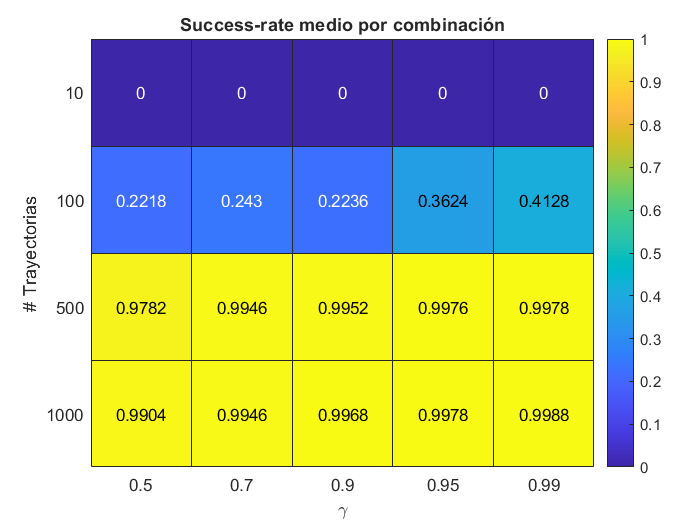
\includegraphics[width=0.7\textwidth]{../../experiments/directEstimation/experiment-1/results/success.png}
    \caption{Tasa de éxito para diferentes combinaciones de $\gamma$ y \textit{número de trayectorias}}
    \label{fig:directEstimation-success}
\end{figure}

Se puede observar que el parámetro que más afecta a la tasa de éxito es el \textit{número de trayectorias}. A medida que aumenta el número de trayectorias, la tasa de éxito también aumenta. Sin embargo, el factor de descuento no parece tener un efecto significativo en la tasa de éxito.

\

El mejor resultado se obtiene con un \textit{número de trayectorias} de 1000 y un factor de descuento de 0.99, donde el algoritmo alcanza una tasa de éxito de aproximadamente el 99.9\%.

\

\textbf{Recompensa media y número de pasos medios}

\begin{figure}[H]
    \centering
    \begin{subfigure}{0.7\textwidth}
        \centering
        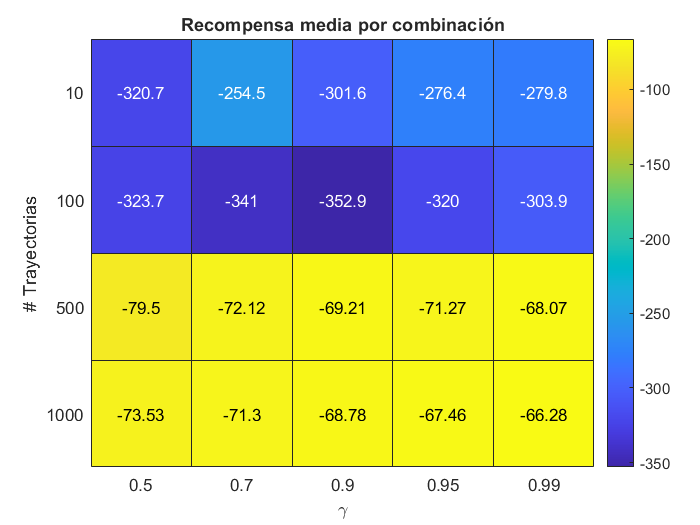
\includegraphics[width=\textwidth]{../../experiments/directEstimation/experiment-1/results/reward.png}
        \caption{Recompensa media para diferentes combinaciones de $\gamma$ y \textit{número de trayectorias}}
        \label{fig:directEstimation-subfig-reward}
    \end{subfigure}
    \hfill
    \begin{subfigure}{0.7\textwidth}
        \centering
        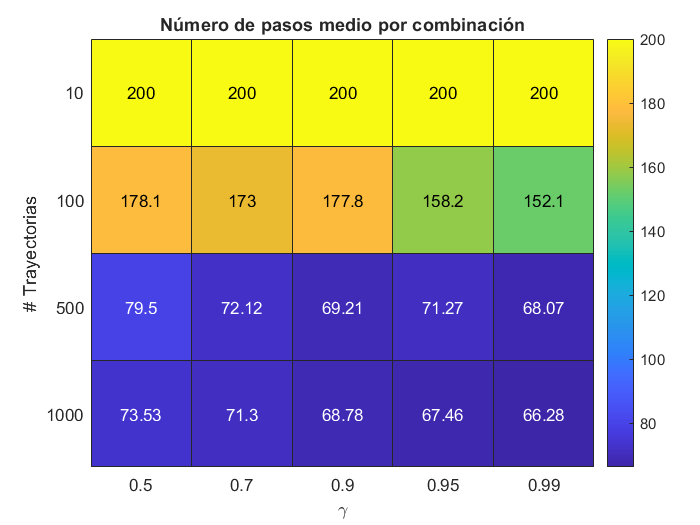
\includegraphics[width=\textwidth]{../../experiments/directEstimation/experiment-1/results/steps.png}
        \caption{Número de pasos para diferentes combinaciones de $\gamma$ y \textit{número de trayectorias}}
        \label{fig:directEstimation-subfig-steps}
    \end{subfigure}
    \caption{Análisis de la recompensa media y número de pasos}
    \label{fig:directEstimation-reward}
\end{figure}

El análisis de la recompensa media y el número medio de pasos revela que:

\begin{itemize}
    \item Las recompensas mejoran significativamente (son menos negativas) al aumentar el \textit{número de trayectorias} y, por lo tanto, el número de pasos también se reduce. 
    \item El factor de descuento tiene un efecto menos significativo en la recompensa media y el número de pasos, todo y que se observa que $\gamma$ inferiores a 0.9 tienden a tener una recompensa media mejor.
    \item Las mejores recompensas se obtienen con $\gamma \geq 0.99$, y con un \textit{número de trayectorias} de 1000.
\end{itemize}

La combinación óptima es $\gamma = 0.99$, \textit{número de trayectorias} = 1000 y logra una recompensa media de -66.28. Corresponde con la combinación que obtiene mejor tasa de éxito. 
\\

Se puede observar que el número medio de pasos corresponde exactamente con la recompensa media en cada configuración. Esto nos indica que el agente no cae por el barranco en ningún momento, ya que sino la recompensa media sería más negativa (-100 de recompensa por caer en 1 paso, perderia la correspondencia de -1 de recompensa por cada paso).

\

La hipótesis inicial de que un mayor número de trayectorias y un mayor factor de descuento mejoran el rendimiento del algoritmo se confirma. Sin embargo, el número de trayectorias parece tener un efecto más significativo que el factor de descuento.

\

\textbf{Tiempo de entrenamiento}

\

Para el tiempo de entrenamiento, se han elegido las tres combinaciones que mejor rendimiento han dado. 

\begin{figure}[H]
    \centering
    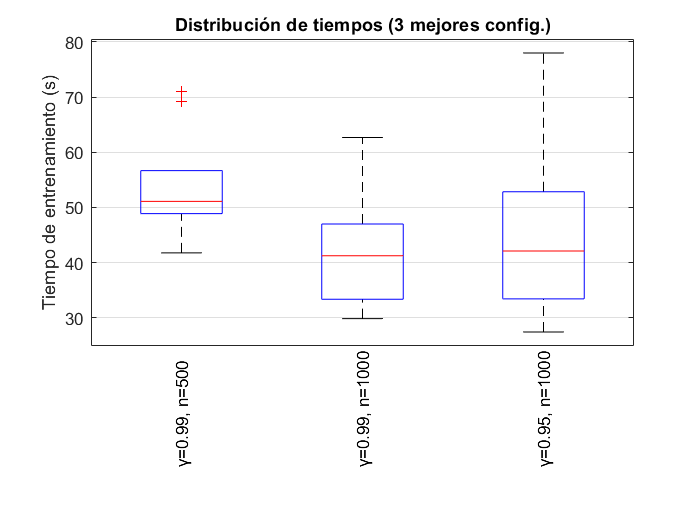
\includegraphics[width=0.8\textwidth]{../../experiments/directEstimation/experiment-1/results/time.png}
    \caption{Tiempo de entrenamiento para diferentes combinaciones de $\gamma$ y \textit{número de trayectorias}}
    \label{fig:directEstimation-time}
\end{figure}

El tiempo de entrenamiento medio resulta ser el mejor para la solución con mejor tasa de éxito y recompensa media. Este es de media de 42.42 segundos, con un intervalo de confianza del 95\% de [34.75,  50.09] segundos. Los demás tiempos del gráfico son los siguientes: 44.95 segundos con IC 95\% [33.92,  55.99] para $\gamma = 0.95$ y \textit{número de trayectorias} = 1000, y 53.89 segundos con IC 95\% [47.35,  60.44] para $\gamma = 0.99$ y \textit{número de trayectorias} = 500.

\subsubsection{Experimento número de episodios de entrenamiento}

\paragraph{Diseño experimental}

El objetivo de este experimento es analizar el rendimiento del algoritmo \textit{Direct Estimation} en función del número de episodios de entrenamiento.

\begin{table}[H]
    \centering
    \begin{tabularx}{\textwidth}{|p{4cm}|X|} % Especificar el ancho de las columnas
        \hline % Línea horizontal superior
        \textbf{Observación} & El rendimiento del algoritmo varía con el número de episodios de entrenamiento.
        \\ \hline
        \textbf{Planteamiento} & Se compara la tasa de acierto (llegar al estado final), la recompensa media, número de pasos y tiempo de entrenamiento del algoritmo para diferentes números de episodios de entrenamiento.
        \\ \hline
        \textbf{Hipótesis} & Un mayor número de episodios de entrenamiento mejorará el rendimiento del algoritmo.
        \\ \hline
        \textbf{Método} & 
        \begin{itemize}
            \item Se fijan los mejores valores para \(\gamma\) y \textit{número de trayectorias} del experimento anterior.
            \item Se eligen los siguientes valores para \textit{número de episodios de entrenamiento}: \textit{número de episodios de entrenamiento} \(\in \{100, 500, 1000, 5000\}\).
            \item Para cada \textit{número de episodios}, se ejecuta el algoritmo \textit{Direct Estimation} en el entorno.
            \item Se evalúa la política obtenida probándola con 500 episodios.
            \item Se repite el proceso para cada \textit{número de episodios} 10 veces.
        \end{itemize}
        \\ \hline
    \end{tabularx}
    \caption{Direct Estimation - Experimento 2 - Número de episodios de entrenamiento}
    \label{tab:diseñoDirectEstimationExp2}
\end{table}

\paragraph{Resultados}

\subsubsection{Experimento Patience}

\paragraph{Diseño experimental}

El objetivo de este experimento es ver si el algoritmo \textit{Direct Estimation} puede detenerse antes de que se alcance el número máximo de episodios de entrenamiento, lo que podría reducir el tiempo de entrenamiento sin afectar el rendimiento.

\begin{table}[H]
    \centering
    \begin{tabularx}{\textwidth}{|p{4cm}|X|} % Especificar el ancho de las columnas
        \hline % Línea horizontal superior
        \textbf{Observación} & El algoritmo \textit{Direct Estimation} tiene fases largas de entrenamiento sin mejora.
        \\ \hline
        \textbf{Planteamiento} & Se compara la tasa de acierto (llegar al estado final), la recompensa media, número de pasos y tiempo de entrenamiento del algoritmo para diferentes valores de iteraciones sin mejora para detener el entrenamiento (\textit{patience}).
        \\ \hline
        \textbf{Hipótesis} & Un valor de \textit{patience} más bajo permitirá al algoritmo detenerse antes y reducir el tiempo de entrenamiento sin afectar significativamente el rendimiento.
        \\ \hline
        \textbf{Método} & 
        \begin{itemize}
            \item Se fijan los mejores valores para \(\gamma\), \textit{número de trayectorias} y \textit{número de episodios de entrenamiento} de los experimentos anteriores.
            \item Se eligen los siguientes valores para \textit{patience}: \textit{patience} \(\in \{10, 100, 1000\}\).
            \item Para cada \textit{patience}, se ejecuta el algoritmo \textit{Direct Estimation} en el entorno.
            \item Se evalúa la política obtenida probándola con 500 episodios.
            \item Se repite el proceso para cada \textit{patience} 10 veces.
        \end{itemize}
        \\ \hline
    \end{tabularx}
    \caption{Direct Estimation - Experimento 3 - Patience}
    \label{tab:diseñoDirectEstimationExp3}
\end{table}

\paragraph{Resultados}